\section{Model Parametrization}
\label{sec:model_parametrization}

\jb{This section copy whole detailed material research paragraphs from the report, we need to drasticaly 
reduce this text, while preserving references to the value resources.}
\subsection{Site-Specific Data}
\label{sec:site_specific_data}

\subsubsection{Geological context}

\par The geological context of the \URFBII is rooted in the complex
geomechanics of the 12\textsuperscript{th} level of the
% \href{https://www.google.com/url?sa=t&rct=j&q=&esrc=s&source=web&cd=&ved=2ahUKEwj_x4Xo1OaOAxWpQ_EDHYluA8IQFnoECB4QAQ&url=https%3A%2F%2Fmineralexpert.org%2Farticle%2Frozna-uranium-mine&usg=AOvVaw0CJNZxChFCpxJT_Fe9Y5V7&opi=89978449}{Rožná}
\Rozna mine in the Czech Republic, situated approximately 500--600 meters
below the earth's surface.
The research facility consists of several galleries, each approximately
70--90 m long, accessed from the main transport gallery P\v S1-123, see
Fig. \ref{fig:mapa}.
\begin{figure}
    \centering
    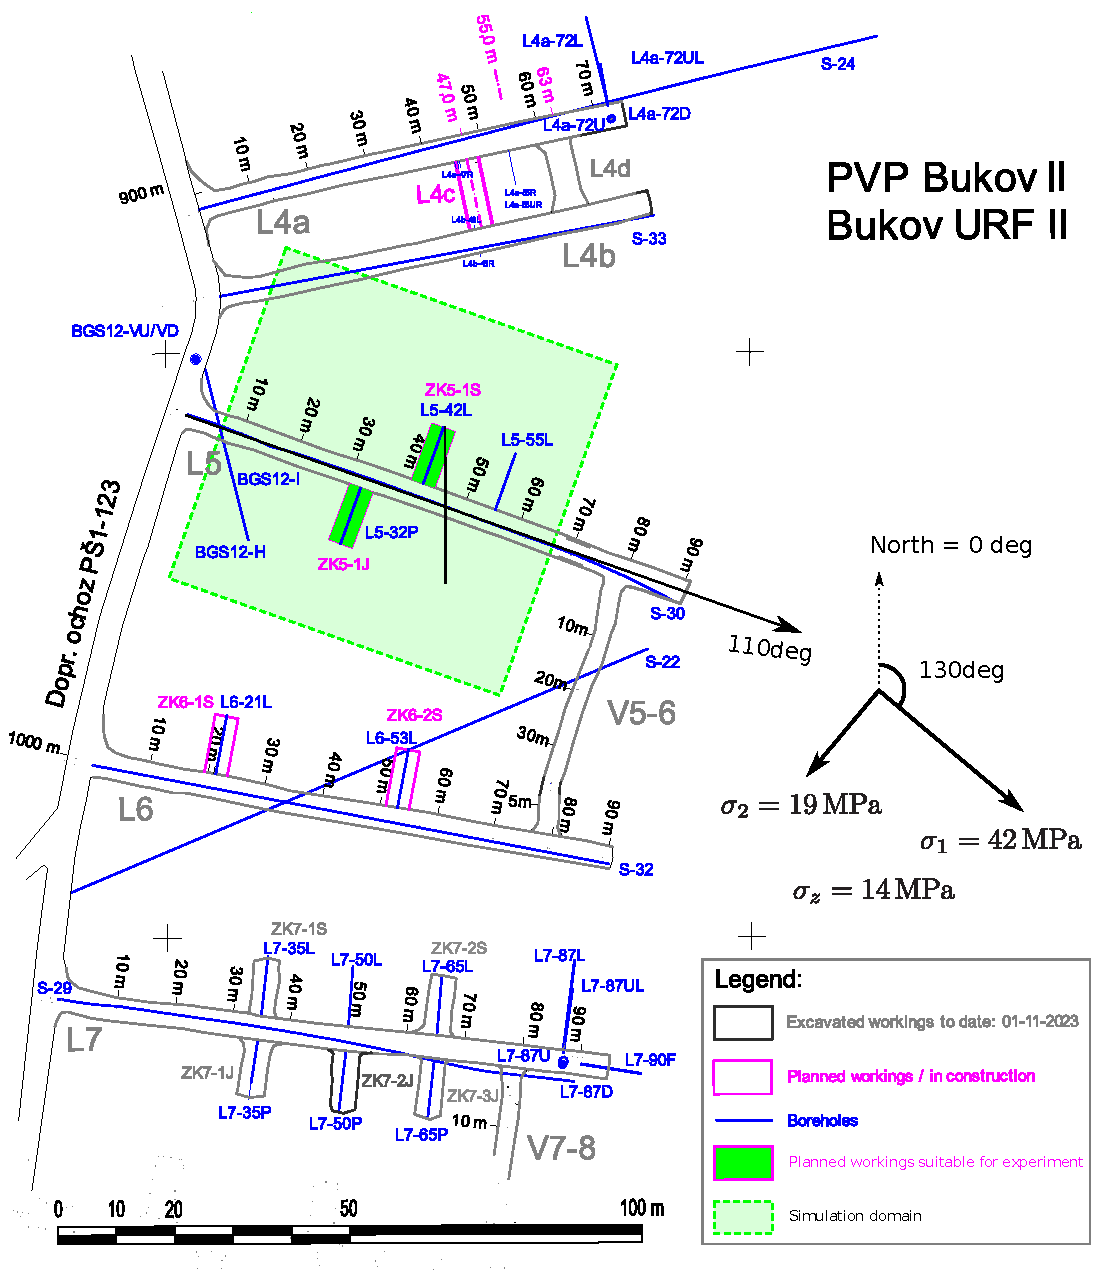
\includegraphics[width=\textwidth]{graphics/mapa_en.pdf}
    \caption{Situation plan of \URFBII.}
    \label{fig:mapa}
\end{figure}
The zone of interest is around the L5 laboratory gallery and the adjacent 10 m
long ZK5-1J and ZK5-1S test chambers.

\par The geology here is heavily influenced by metamorphic processes, with
structural foliation affecting mechanical and hydraulic properties.

\par Mechanically, the rock mass exhibits properties influenced by its
foliation, as evidenced by uniaxial, cyclic loading, and triaxial tests
performed on core samples. The elastic modulus varies considerably based on
orientation relative to foliation (orthogonal, parallel, or skewed).
Measurements include deformation modulus values up to 71.9 GPa and uniaxial
compressive strengths reaching 231 MPa (\cite{Bukovska2025}).
\par Cyclic and triaxial tests revealed complex stress-strain behavior, with
the Hoek-Brown criterion providing a framework for strength characterization.

\paragraph{Geological materials.}
% \subsection{Geological Model and Lithologies}
% The numerical model incorporates a new mesh derived from a highly detailed

According to a detailed geological model created by the Czech Geological Survey
(\cite{Bukovska2025final}), the lithologies present at the site primarily
include:
\begin{itemize}%[noitemsep]
    \item Migmatitized amphibolite,
    \item Migmatite,
    \item Biotite-Amphibole paragneiss migmatitized.
\end{itemize}
An illustration of the material layout in the surrounding of the \gls{L5} is
depicted in Fig. \ref{fig:geological_mesh}.

\begin{figure}%[H]
    \centering
    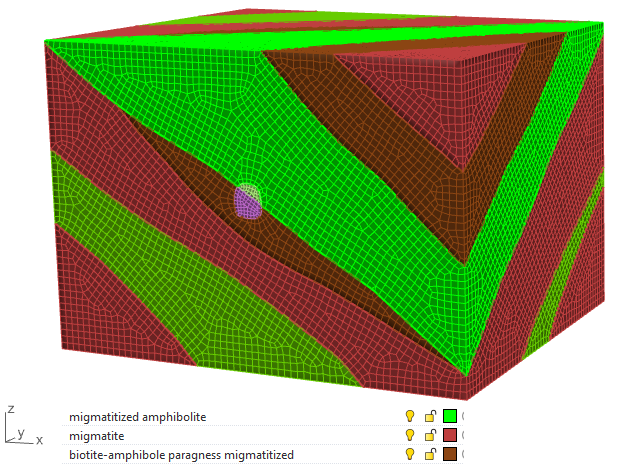
\includegraphics[width=0.5\textwidth]{graphics/plasticity/geological_mesh.png} % Example image path
    % \caption{Mesh used in this study compromising the detailed geological setting.}
    \caption{Structure of geological materials in the zone of interest.}
    \label{fig:geological_mesh}
\end{figure}

%%% po sem preneseno z kap. od Felipeho

\subsubsection{Hydraulic conductivity}
\label{sec:hydro_cond}
Within the Characterization Project, water-pressure tests were conducted in
boreholes at \URFBII. Laboratory measurements on rock samples from the
12\textsuperscript{th}--24\textsuperscript{th} levels of the \Rozna were also
performed as part of the Deep Horizons Project. This section summarizes the
reported values of hydraulic conductivity. All values refer to the apparent
hydraulic conductivity of rock samples and rock mass; however, some
measurements---particularly in situ tests---may be significantly influenced by
the presence of discrete fractures.

In \cite{tz_char_1}, Sec. 2.4.1, a general characterization of the site states
that:
%
\begin{center}
\begin{minipage}{0.8\textwidth}
\it \textquote{In the permeable zones of the \Rozna (with the presence of open
fractures), one can expect hydraulic conductivity of magnitude
$10^{-7}-10^{-6}$ \mps.
In moderately fractured zones, hydraulic conductivity ranges between
$10^{-11}-10^{-8}$ \mps.
Hydraulic conductivity of the rock matrix is of order $10^{-13}-10^{-11}$ \mps.
The above-mentioned values are valid at the scale of the performed tests, i.e.
on the order of meters.

It is also necessary to take into account the specific conditions of the mine,
where the tests are performed in partially saturated rock mass with uncertain
pressure conditions around the tested boreholes.
In the rock mass undisturbed by the excavation works one can therefore expect
lower values of hydraulic conductivity.}
\end{minipage}
\end{center}
%
Besides this characterization, we collected results from in-situ as well as
laboratory measurements:
\begin{itemize}
\item Water pressure tests in the vicinity of the L5 gallery. The measured
hydraulic conductivities in the boreholes L5-50UL, L5-49DL, L5-37UR, L5-37R,
L5-22DR, L5-24DR, L5-23UR and L5-26R are reported in \cite{tz_monitoring},
Tab. 4 on p. 18-19. Their values are in the range
$\num{2.13e-11}-\num{8.78e-10}$ \mps.

\item Water pressure tests in the vicinity of the L7 and L8 galleries. The
measured hydraulic conductivities in the boreholes L7-35P, L7-50P, L7-87D, and
L8-54DL are reported in \cite{tz_char_2}, Tab. 12 on p. 86. Their values are
in the range $\num{4.5e-13}-\num{3.4e-10}$ \mps.

\item Water pressure tests in the vicinity of the L4b and L8 galleries. The
measured hydraulic conductivities in the boreholes S-33, L4-73D and L8-54DL
(with more detailed segment measurements in comparison to \cite{tz_char_2}) are
reported in \cite{tz_char_3}, Tab. 10--11 on p. 86. The values are in the range
$\num{3.7e-12}-\num{3.8e-9}$ \mps ~for S-33 and L4-73D, and
$\num{2e-10}-\num{5.1e-10}$ \mps ~for L8-54DL, respectively.

\item Laboratory measurements on samples from level 12. In particular, one
large-volume sample (V-12) and two core samples (BGS12-VD and BGS12-I) from
the vicinity of \URFBI were analyzed, see Fig. 10 in \cite{tz_hh}.
In the case of V-12, specimens were prepared in three directions with respect
to metamorphic foliation: orthogonal (K), parallel (P) and slanted (S).
The measured values are reported in \cite{tz_hh}, Tab. 16, 26 and 34 in
Sec. 2.3.5.3.
\end{itemize}

The collected values of hydraulic conductivity are summarized in the following
two tables.
In-situ measurements are presented in Tab. \ref{tab:hydr_cond}, while data from
laboratory testing are in Tab. \ref{tab:hydr_cond_lab}.

\scriptsize
\begin{longtable}{@{}lrrSr@{}}
\caption{In-situ measurements of hydraulic conductivity.}\label{tab:hydr_cond}\\
\toprule
Location &Borehole &Orientation &{Hydraulic conductivity} &Data source \\%\cmidrule{1-5}
&/sample & &\mps & \\\midrule
\endfirsthead
\caption{In-situ measurements of hydraulic conductivity (continued).}\\
\toprule
Location &Borehole &Orientation &{Hydraulic conductivity} &Data source \\%\cmidrule{1-5}
&/sample & &\mps & \\\midrule
\endhead
\multirow{8}{*}{L4b} &\multirow{3}{*}{S-33} &\multirow{3}{*}{} &2.60e-10 &\multirow{8}{*}{\cite{tz_char_3}, Tab. 10 $ $} \\
& & &8.80e-10 & \\
& & &3.80e-9 & \\\cmidrule{2-4}
&\multirow{5}{*}{L4-73D} &\multirow{5}{*}{} &3.70e-12  \\
& & &3.90e-11 & \\
& & &4.70e-11 & \\
& & &6.50e-11 & \\
& & &7.80e-11 & \\\midrule
\multirow{23}{*}{L5} &\multirow{3}{*}{L5-50UL} &\multirow{3}{*}{} &1.69e-10 &\multirow{23}{*}{\cite{tz_monitoring}, Tab. 4 $ $} \\
& & &1.53e-10 & \\
& & &1.34e-10 & \\\cmidrule{2-4}
&\multirow{6}{*}{L5-49DL} &\multirow{6}{*}{} &7.65e-10 \\
& & &6.01e-10 & \\
& & &4.81e-10 & \\
& & &7.25e-10 & \\
& & &7.05e-10 & \\
& & &8.78e-10 & \\\cmidrule{2-4}
&\multirow{4}{*}{L5-37UR} &\multirow{4}{*}{} &1.88e-10  \\
& & &2.32e-10 & \\
& & &1.29e-10 & \\
& & &1.86e-10 & \\\cmidrule{2-4}
&\multirow{3}{*}{L5-37R} &\multirow{3}{*}{} &8.95e-11  \\
& & &6.72e-11 & \\
& & &7.83e-11 & \\
&L5-22DR & &9.36e-11  \\
&L5-24DR & &9.36e-11  \\\cmidrule{2-4}
&\multirow{3}{*}{L5-23UR} &\multirow{3}{*}{} &4.68e-11  \\
& & &4.68e-11 & \\
& & &2.34e-11 & \\\cmidrule{2-4}
&\multirow{3}{*}{L5-26R} &\multirow{3}{*}{} &8.51e-11  \\
& & &4.26e-11 & \\
& & &2.13e-11 & \\\midrule
\multirow{7}{*}{L7} &L7-35P & &4.80e-11 &\multirow{7}{*}{\cite{tz_char_2}, Tab. 12 $ $} \\\cmidrule{2-4}
&L7-50P & &5.10e-11 & \\\cmidrule{2-4}
&\multirow{5}{*}{L7-87D} &\multirow{5}{*}{} &3.50e-13 & \\
& & &4.50e-13 & \\
& & &5.40e-13 & \\
& & &8.70e-13 & \\
& & &1.60e-12 & \\\midrule
\multirow{5}{*}{L8} &\multirow{5}{*}{L8-54DL} &\multirow{5}{*}{} &2.00e-10 &\multirow{5}{*}{\cite{tz_char_2}, Tab. 11 $ $} \\
& & &3.00e-10 & \\
& & &3.30e-10 & \\
& & &3.40e-10 & \\
& & &5.10e-10 & \\
\bottomrule
% \end{tabular}
\end{longtable}
\normalsize

\scriptsize
\begin{longtable}{@{}lrSr@{}}
\caption{Laboratory measurements of hydraulic conductivity.}\label{tab:hydr_cond_lab}\\
\toprule
Borehole &Orientation &{Hydraulic conductivity} &Data source \\%\cmidrule{1-5}
/sample & &\mps & \\\midrule
\endhead
\multirow{7}{*}{V-12} &K &8.80e-14 &\multirow{7}{*}{\cite{tz_hh}, Tab. 16 $ $} \\
&P &1.20e-13 & \\
&P &1.20e-13 & \\
&P &1.70e-13 & \\
&S &2.10e-13 & \\
&S &4.30e-13 & \\
&S &4.50e-13 & \\\cmidrule{1-4}
\multirow{3}{*}{BGS12-VD} &\multirow{3}{*}{} &3.50e-13 &\multirow{3}{*}{\cite{tz_hh}, Tab. 26 $ $} \\
& &3.60e-13 & \\
& &8.30e-9 & \\\cmidrule{1-4}
\multirow{3}{*}{BGS12-I} &\multirow{3}{*}{} &2.71e-13 &\multirow{3}{*}{\cite{tz_hh}, Tab. 34 $ $} \\
& &2.75e-13 & \\
& &1.09e-12 & \\
\bottomrule
% \end{tabular}
\end{longtable}
\normalsize

\subsubsection{Storativity, porosity and Biot-Willis coefficient}
\label{sec:storativity}
For the computation of storativity [\unit{\per\meter}] by the formula
\[ S = \varrho_w g (\beta_s + \phi \beta_w), \quad \beta_s=(\alpha-\phi)(1-\alpha)/K, \quad K = E/(3(1-2\nu)), \]
(see e.g. \cite{freeze1979groundwater}), the additional knowledge of the
following quantities is needed: porosity $\phi$ and Biot-Willis coefficient
$\alpha$ of the rock massif, density $\varrho_w$ and  compressibility $\beta_w$
of water.

We have collected the following values for \URFBII (see Tab. \ref{tab:dens_por}
for the list):
\begin{itemize}
    \item Density and porosity in L7 (\cite{tz_char_1}, Tab. 8 and 9);
    \item Density and porosity in L6 (\cite{tz_char_2}, Tab. 14);
    \item Density in L5 (\cite{tz_char_3}, Tab. 12);
    \item Density and porosity in the large-volume sample V-12
    (\cite{tz_hh}, Tab. 14 and 15).
\end{itemize}

\begin{table}[!htp]\centering
\caption{Measurements of density and porosity.}\label{tab:dens_por}
\scriptsize
\begin{tabular}{lrrrrrrr}\toprule
Location &Sample &Density &
\makecell[c]{Total\\ porosity} &
\makecell[c]{Open\\ porosity} &
\makecell[c]{Porosity\\ by MIP} &Data source \\%\cmidrule{1-7}
& &kg m${}^{-3}$ &\% &\% &\% & \\\midrule
L7 &16962 &2897 &0.89 &0.13 &0.16 &\cite{tz_char_1}, Tab. 8-9 $ $ \\
L6 &17074 &2745 &1.13 &0.62 &0.75 &\cite{tz_char_2}, Tab. 14-15 $ $ \\
L5 &17363 &2930 & & & &\cite{tz_char_3}, Tab. 12 $ $ \\
\parbox{1cm}{\URFBIIm} &V-12/16432 &2765 &3.23 &0.96 &0.3 &\cite{tz_hh}, Tab. 14-15 $ $ \\
\bottomrule
\end{tabular}
\end{table}

Based on the data summarized in Table~\ref{tab:dens_por}, the investigated rock
massif in \URFBII\ exhibits very low porosity, with total porosity mostly
between 1-3~\% and open porosity generally below 1~\%. Such values are
characteristic of compact crystalline and metamorphic rocks and indicate
limited pore volume contributing to fluid storage. For modelling purposes, a
representative matrix porosity in the range
\[ \phi\approx 0.001-0.02 \]
can be adopted.

The Biot–Willis coefficient $\alpha$ is defined as
\[ \alpha = 1-\frac{K_D}{K_S}, \]
where $K_D$ is the drained bulk modulus of the rock and $K_S$ the bulk modulus
of the solid phase. In low-porosity, high-stiffness crystalline rocks, $K_D$
approaches $K_S$, leading to relatively small $\alpha$ values. Experimental
studies on dense crystalline and low-porosity rocks typically report $\alpha$
in the range
\[ \alpha\approx0.1-0.3, \]
which is significantly lower than in porous sedimentary formations.

Considering the measured porosity, the high stiffness of the metamorphic rocks
at the site of Rožná/Bukov, and published poromechanical data for similar
lithologies, this range is regarded as mechanically consistent for the intact
rock matrix. Using representative elastic parameters and water properties, the
resulting storativity is of the order
\[ S\approx 10^{-7}-10^{-5}~ \unit{\per\meter}, \]
which is typical for low-permeability crystalline rock environments.

\subsubsection{Transport parameters}
\label{sec:review_diffusion}
Effective diffusivity has been determined by laboratory measurements on
large-volume samples from 12\textsuperscript{th} floor of \URFBI. Two methods
were employed, namely the analytical solution and the time-lag method
(\cite{tz_hh}).
The obtained values are reported in Tab. \ref{tab:diffusivity}.

\begin{table}[!htp]\centering
\caption{Measurements of effective diffusivity.}\label{tab:diffusivity}
\scriptsize
\begin{tabular}{lrrrrrr}\toprule
Sample &Porosity &\multicolumn{3}{c}{Effective diffusivity} &Data source \\
&\% &\multicolumn{3}{c}{$\cdot10^{-13}$ m${}^2$s${}^{-1}$} & \\\midrule
& &${}^3$H &${}^{36}$Cl &${}^{125}$I & \\
\midrule
\multirow{2}{*}{V12\_K21\_4} &\multirow{2}{*}{0.66} &2.7 &0.6 & &\multirow{8}{*}{\cite{tz_hh}, Tab. 133 $ $} \\
& &3 &0.4 & & \\\cmidrule{1-5}
\multirow{2}{*}{V12\_K21\_7} &\multirow{2}{*}{0.57} &5 & &1.6 & \\
& &4.3 & &1.6 & \\\cmidrule{1-5}
\multirow{2}{*}{V12\_P19\_2} &\multirow{2}{*}{1.2} &9.2 &4.4 & & \\
& &9.6 &3.4 & & \\\cmidrule{1-5}
\multirow{2}{*}{V12\_P19\_3} &\multirow{2}{*}{1.36} &11.7 & &3.1 & \\
& &9.8 & &2.4 & \\
\bottomrule
\end{tabular}
\end{table}

\subsubsection{Backfill and its expected properties}

The access tunnel will be filled mechanically. The filling machine will
transport the pelletized material from the transport containers to the
placement location using pneumatic (blowing) or mechanical transport (belt,
screw conveyor). If necessary, the machine will perform working lining of the
tunnel and/or vibratory compaction during execution. It is assumed that the
access tunnel will be gradually filled from its previously closed end towards
the future plug.

The backfill material must ensure that there is no excessive displacement of
the material from the disposal well (sufficient support against swelling of the
buffer). It must also ensure that the transport of water and radionuclides
through the backfill is minimized. However, at the same time, it must allow gas
to escape from the buffer without impairing the function of the backfill.

The backfill for the Czech deposition concept is made from the pelletized
\acrshort{BCV} bentonite. To achieve the aforementioned requirements, the
following backfill and pellet parameters have been suggested in
\cite{Svoboda2023navrh}:

\noindent
\textbf{Backfill:}
\begin{itemize}
    \item Average dry density after placement to the access tunnels:
    $\rho_d=1400\,$kg/m$^3$;
    \item Moisture after placement: value not yet determined;
    \item Form: pellets.
\end{itemize}
\textbf{Pellets:}
\begin{itemize}
    \item Dry density: more than $2000\,$kg/m$^3$;
    \item Moisture: value not yet determined;
    \item Grain size: not yet determined.
\end{itemize}

\subsubsection{Evaluation of hydraulic conductivity and swelling pressure}

The next aim was to analyze the dependence of hydraulic conductivity and
swelling pressure on the average dry density of M182. For this study, only the
M182 0-8 mm material was used, see \cite{Stastka2020navrh} . The evaluation was
conducted in accordance with the supplier's internal methodologies, based on
valid technical standards. However, the swelling pressure tests were not
completed in a standard manner, and therefore it was necessary to determine the
swelling pressure by reducing the total stress from the conclusion of the test
(by approximately $3-15~\%$).

The~dependence of hydraulic conductivity on the average dry density is depicted
in Fig.~\ref{fig:image_hyd_vod}. The trend indicates that increasing dry
density leads to decreasing hydraulic conductivity.
\begin{figure}[!htbp]
  \centering
  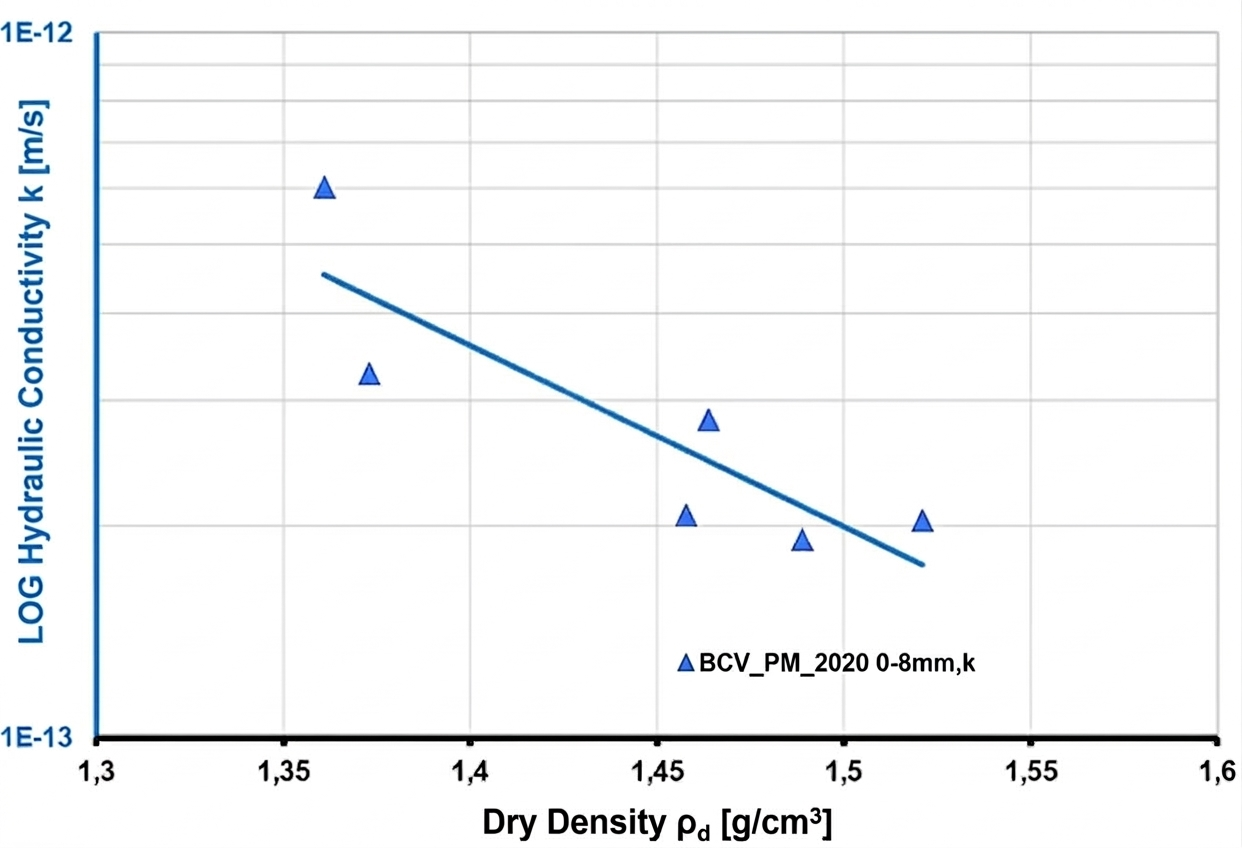
\includegraphics[width=0.8\textwidth]{graphics/img_ugn/Cimage_hyd_vod.png}
  \caption{Dependence of hydraulic conductivity $k$ (logarithmic scale) on dry
  density \(\rho_d\) for bentonite material \texttt{\acrshort{m182-0-8}}.}
  \label{fig:image_hyd_vod}
\end{figure}

The graph in Figure~\ref{fig:image14} illustrates the relationship between the
dry density \(\rho_d\) and the swelling pressure \(\sigma_\text{sw}\) of
M182 0-8 mm. As the dry density increases from approximately
1.3~g/cm\(^3\) to 1.5~g/cm\(^3\), a significant rise in the swelling pressure
is observed, with maximum values exceeding 6~MPa. The fitted curve suggests an
exponential dependency, highlighting that even minor increases in dry density
result in considerable improvements in swelling pressure.

\begin{figure}[!htbp]
  \centering
  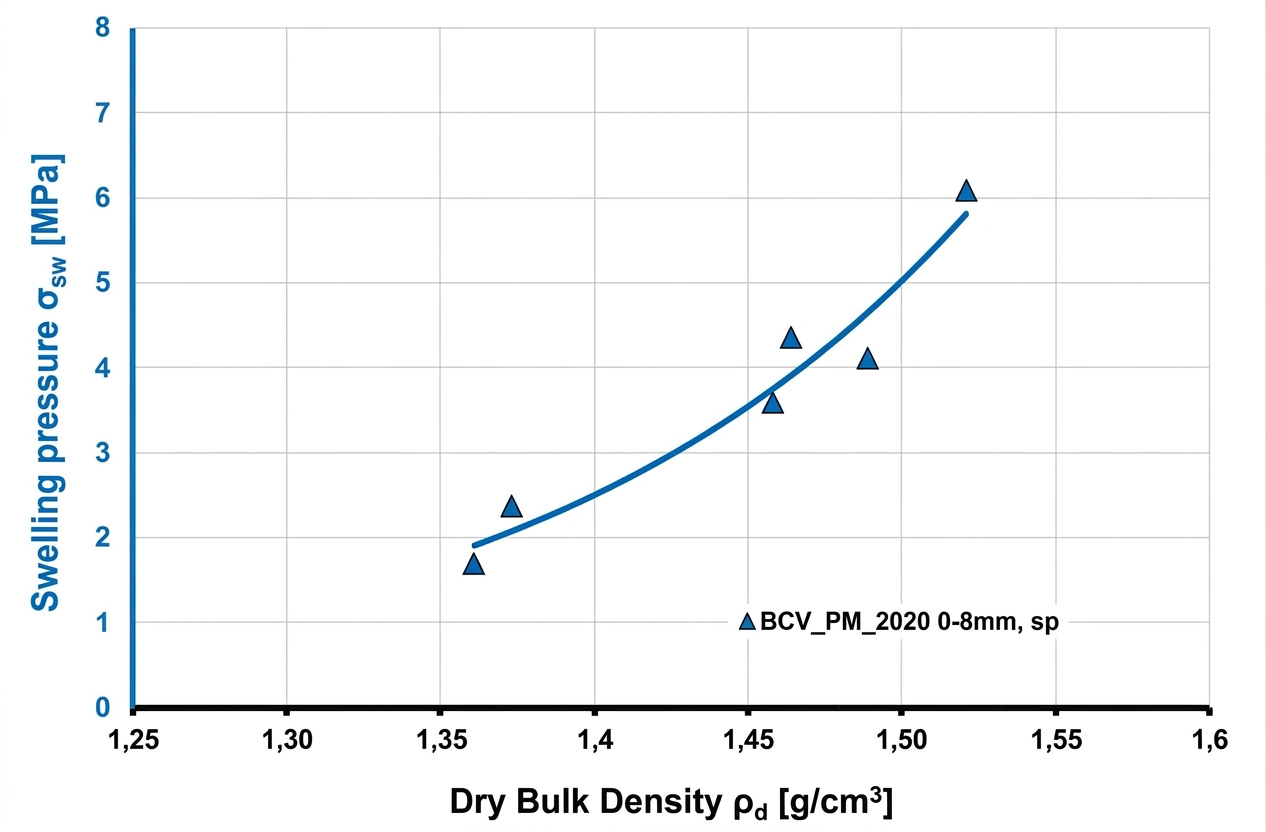
\includegraphics[width=0.8\textwidth]{graphics/img_ugn/Cimage14.png}
  \caption{Dependence of swelling pressure \(\sigma_\text{sw}\) on dry density
  \(\rho_d\) for pelletized bentonite material \texttt{\acrshort{m182-0-8}}.
  The swelling pressure increases significantly with higher dry density.}
  \label{fig:image14}
\end{figure}

This behavior confirms that the developed pelletized bentonite material
exhibits the required properties for use as a buffer and sealing component in
the construction of deep geological repositories for radioactive waste. The
combination of high swelling pressure and appropriate grain size distribution
ensures effective mechanical stability and minimizes potential pathways for
radionuclide migration.

Furthermore, Figure~\ref{fig:image15} presents a comparative analysis of the
hydro-mechanical behavior of pelletized and initial non-pelletized bentonite.
These two materials are denoted as \texttt{M182 0-8 BCV\_PM\_2020} and
\texttt{BCV\_PM\_2017} within this study. For \texttt{BCV\_PM\_2017}, data from
\cite{Cervinka2018kompletni,Svoboda2019interakcni} were used. The left vertical
axis shows the hydraulic conductivity plotted on a logarithmic scale, while the
right vertical axis corresponds to the swelling pressure.

\begin{figure}[!htbp]
  \centering
  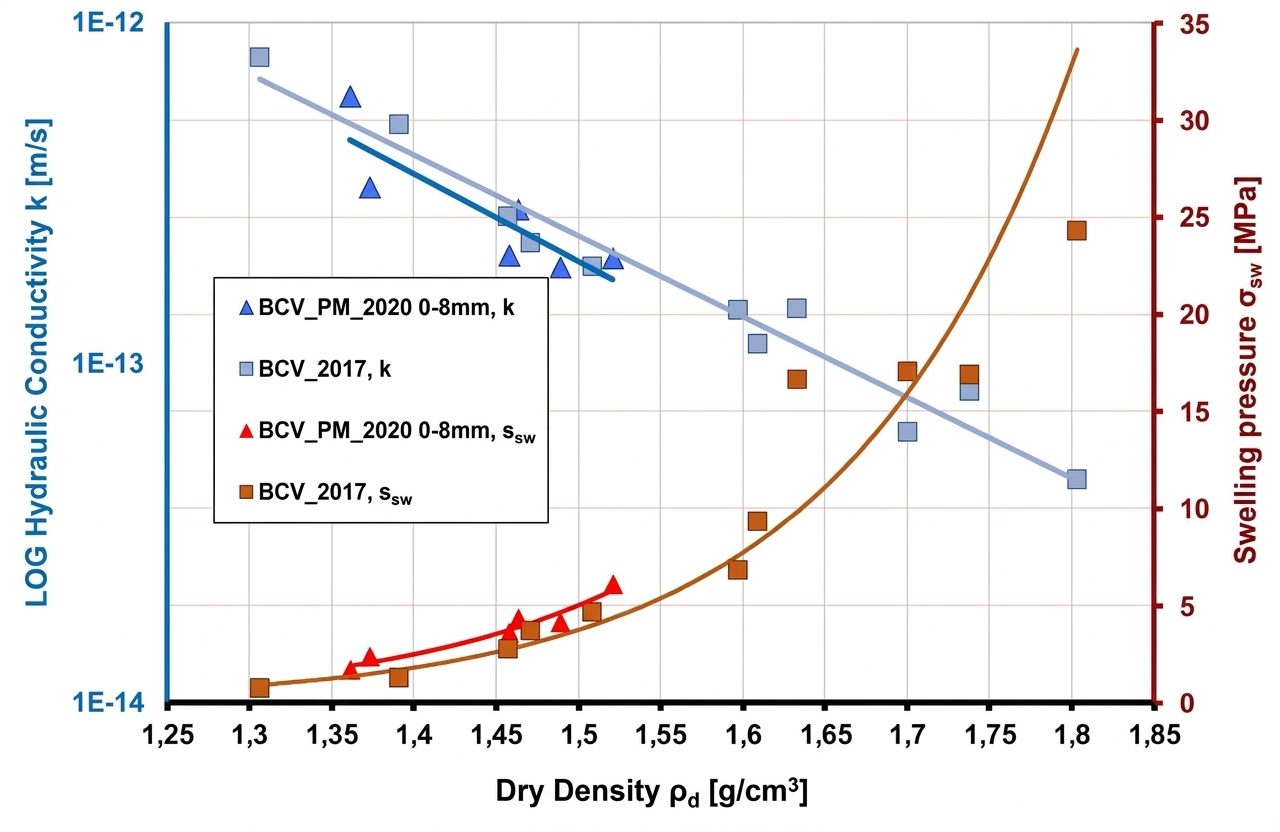
\includegraphics[width=0.8\textwidth]{graphics/img_ugn/Cimage15.png}
\caption{Comparison of the relationship between dry density \(\rho_d\) and
hydraulic conductivity $k$ (left axis) and swelling pressure (right axis) for
pelletized bentonite materials BCV\_PM\_2020. Results are compared to
non-pelletized ground bentonite BCV\_2017.}
  \label{fig:image15}
\end{figure}

The results (dependencies) for both compared materials appear to be similar.
For both materials, a clear trend is observed in which an increase in dry
density \(\rho_d\) results in a significant reduction in hydraulic conductivity
and a simultaneous exponential increase in swelling pressure. The
\texttt{M182 0-8 BCV\_PM\_2020} material exhibits slightly lower hydraulic
conductivity and relatively moderate swelling pressures compared to the
\texttt{BCV\_PM\_2017} material across the range of densities tested. This
indicates that the pelletized bentonite (\texttt{BCV\_PM\_2020}) has favorable
properties for use as a backfill material in deep geological repositories for
radioactive waste, combining low permeability with adequate swelling capacity.

Finally, it is important to highlight that all hydraulic conductivity and
swelling-pressure tests reported in Figs.~\ref{fig:image_hyd_vod}–\ref{fig:image15}
were performed under fully saturated conditions (constant-volume saturation).
Therefore, the reported values of
$\sigma_{\text{sw}}$ correspond to the equilibrium swelling pressure in the
saturated state.

\subsubsection{Concluding remarks to achieved hydro-mechanical properties of the BCV pelletized backfill}

Currently, we have the following requirements on the \acrshort{BCV} pelletized
backfill for the Czech deposition concept:
\begin{enumerate}
    \item Dry density of pellets should be greater than $2000 \munit{kg/m^3}$;
    \item Average dry density of the backfill after placement to the access tunnels\\ should be $1400 \munit{kg/m^3}$.
\end{enumerate}
The suggested pellet pressing technology enables us to prepare the pelletized
\texttt{M182 0-8 mm} and \texttt{M182 0-50 mm} materials satisfying the first
requirement. The average dry density of these materials has been analyzed only
via laboratory compaction tests, which is not able to catch the complexity of
in situ conditions. From the performed laboratory experiments, it follows that
the required average density of $1400\,$kg/m$^3$ is achieved for
\texttt{M182 0-50 mm} using all compaction methods. However, for
\texttt{M182 0-8 mm}, only some compaction methods give this required value.

Next, the hydraulic conductivity and swelling pressure of the pelletized BSV
bentonite have been analyzed under laboratory conditions and for the
\texttt{M182 0-8 mm} material.
From these measurements, the hydraulic conductivity and swelling pressure for
fully saturated pellets at an average dry density of
$\rho_d = 1400 \ \mathrm{kg/m^3}$
can be roughly estimated as:
$k = (3.5\text{–}5) \times 10^{-13} \ \mathrm{m/s}, \quad p_s = 1.5\text{–}2.5 \ \mathrm{MPa}$.
For \texttt{M182 0-50 mm}, no measurements of the hydro-mechanical (HM)
parameters of the pellets have been performed. Such measurements could be
helpful from the perspective of possible preferential flow paths (zones with
higher hydraulic conductivity) in the backfill.

The aforementioned analyses are not representative of backfilling emplacement
drifts, where the material will be placed horizontally along irregular tunnel
walls, transported over several tens of meters, and subjected to large-scale
self-compaction, arching, segregation of grain-size fractions, and potential
void formation. A full-scale or large box experiment with horizontal placement
should be used to characterize backfill density distribution, compaction
behavior, and hydro-mechanical properties under realistic geometrical and
operational constraints.

More comprehensive analyses can be found in several international studies. In
the next section, we summarize selected experiences with FEBEX and MX-80
bentonites and related pelletized material. Their knowledge may complete
missing properties of the backfill and may be inspirational for future analyses
of the \acrshort{BCV} pelletized material.

\subsubsection{Transport parameters of saturated pelletized backfill}
\label{sec:transport_pellets}
\label{sec_concept}

This section provides transport parameters for radionuclide modelling in the
\emph{fully hydrated, long-term} state of the pelletized backfill (time scale
$\sim 10^3$~years). Transient resaturation and early-time preferential flow
during hydration are \emph{not} considered. The key design state variable is
the average emplaced dry density $\rho_d$; for the Czech concept we target
$\rho_d \approx 1.4~\mathrm{Mg/m^3}$ (Section~\ref{sec_concept}). Based on the
FEBEX experiment results summarized in Appendix~\ref{sec_append1}, we estimate
an uncertainty range of $\pm 0.1~\mathrm{Mg/m^3}$, corresponding to a standard
deviation $\sigma_{\rho_d}=0.03~\mathrm{Mg/m^3}$. We adopt this convention
throughout, reporting uncertainty either as a
$\pm$ range or explicitly as $\sigma$, taken as one third of the range.

\paragraph{Porosity and pore families (steady, saturated fabric).}
Using the measured solid density of BCV bentonite,
$\rho_s=2.87~\mathrm{Mg/m^3}$, the total porosity is
\[
n = 1-\frac{\rho_d}{\rho_s}\approx 0.51~\pm 0.04 \qquad \text{for}\qquad \rho_d=1.40~\pm 0.1~\mathrm{Mg/m^3}.
\]

\paragraph{Effective diffusion.}
Following \cite{VanLoon2014_NTB1203}, we describe effective pore diffusion
$D_{e}$ in the saturated backfill by an extended
Archie-type relation,
\[
D_{e} \;=\; D_{w}\,\varepsilon^{m_1} \;+\; B\,\varepsilon^{m_2},
\]
where $D_w$ is the diffusivity in the free water
(see Fig. \ref{fig:d_free_water}) and $(m_1,m_2,B)$ are empirical parameter
taken from the compacted-bentonite parameterisation in Tab.~28 of
\cite{VanLoon2014_NTB1203}.
For neutral tracers and most cations, we take
$\varepsilon_i \approx n$ (total porosity). For anions, anion exclusion reduces
the diffusion-accessible porosity; here we treat
$\varepsilon_{\mathrm{an}}$ as bounded and scale the anion-porosity envelope
reported in Tab.~28 to our higher total porosity (dominant uncertainty: ionic
strength and double-layer overlap). For slowly diffusing actinide-like aqueous
complexes we retain the low-mobility envelope from Tab.~28 and scale it with
porosity using the same Archie exponent range.

Using the porosity range stated above and the Tab.~28 parameter envelope, we
provide diffusivity values for species representing four groups: neutral,
 cation, anion, and complex.
The diffusivity at $25^\circ$C is reported via
\[
Y_i \;\equiv\; \log_{10}\!\left(\frac{D_{e,i}}{\mathrm{m^2/s}}\right),
\]
as geometric mean values $Y_{i}$ and log-space standard deviations $\sigma_{i}$:
\begin{align*}
Y_{\mathrm{neu}} &= -9.4,& \sigma_{\mathrm{neu}}&=0.1
\quad \text{(neutral; C$_\mathrm{org}$)},\\
Y_{\mathrm{cat}} &= -9.8,& \sigma_{\mathrm{cat}}&=0.1
\quad \text{(small cation; Ca$^{2+}$)},\\
Y_{\mathrm{an}} &= -10.9,&  \sigma_{\mathrm{an}}&=0.3
\quad \text{(anion; I$^{-}$)},\\
Y_{\mathrm{act}} &= -13.1,& \sigma_{\mathrm{act}}&=0.2
\quad \text{(actinide-like slow complex; Am$^{3+}$)}.
\end{align*}

The larger uncertainty for anions reflects the sensitivity of
$\varepsilon_{\mathrm{an}}$ to porewater chemistry (ionic strength) and
compaction, whereas for neutrals and most cations the uncertainty is dominated
by the (comparatively narrow) porosity range and the Archie-parameter envelope.
\begin{figure}
    \centering
    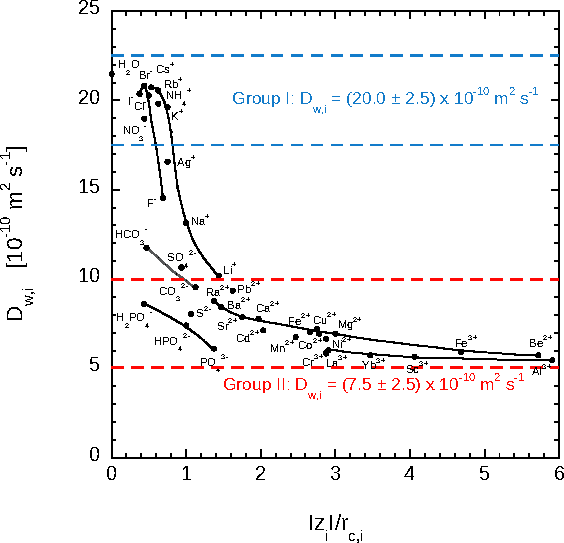
\includegraphics[width=0.6\linewidth]{graphics/free_water_diffusion.pdf}
    \caption{Molecular diffusion in free water, taken from
    \cite{VanLoon2014_NTB1203}.}
    \label{fig:d_free_water}
\end{figure}

\paragraph{Advection and dispersion in the long-term saturated state.}
Following first-order stochastic theory for macroscopic (field-scale)
dispersion (\cite{Zech_Evidence_2023}), we express the longitudinal
macrodispersivity as
\begin{equation}
    \label{eq:dispersivity}
    \alpha_L = \sigma_{\ln K}^2\, I_h,
\end{equation}
where $\sigma_{\ln K}^2=\Var(\ln K)$ is the variance of the log-conductivity
field and $I_h$ is the longitudinal integral scale (defined as the integral of
the normalized correlation function along the mean-flow direction). For the
commonly used exponential correlation model, the integral scale equals the
correlation length parameter, and for other standard correlation models, it is
of the same order.

The variance is dimensionless, in particular it is invariant to
the choice of reference conductivity $K_0$:
\[
 \sigma_{\ln K}^2=\Var(\ln K)=\Var\!\bigl(\ln(K/K_0)\bigr),
\]
since $\Var(\ln K_0)=0$ for a constant $K_0$.

The integral scale is expected to be in the range
$I_h \approx 0.1$--$1~\mathrm{m}$, associated with hydration-related
inhomogeneities. Using the $\rho_d  \propto \log_{10} K$ relation linear fit,
we get:
\[
\sigma_{\log_{10}K} = 6 \sigma_{\rho_d} + 0.08 = 0.26
\]
corresponding to  $\sigma^2_{\ln K}\approx 0.36$.
Then we conclude:
\[
\alpha_L = \sigma_{\ln K}^2 I_h \approx 0.026\text{--}0.26~[m].
\]

\subsection{Determination of \gls{DFN} Parameters Through Bayesian Inversion}
\label{sec:dfn_bayesian_inversion}

\subsubsection{Model parameter distributions}

\paragraph{Aleatory parameters}
The transport model (Section~\ref{sec:transport_model}) is subject to two
sources of aleatory uncertainty:
(i) the random discrete-fracture network, representing geological uncertainty,
and
(ii) numerical uncertainty arising from the construction of the computational
mesh.

For simplicity, we neglect spatial heterogeneity of the material parameters
(caused by unresolved small-scale fractures). We therefore use spatially
constant material parameters, with variability inferred from the observed
in-situ spatial variability. This choice likely overestimates the sensitivity
to these parameters, because true spatial variability would be partly smoothed
by diffusive transport processes and mixing. Other sources of numerical
uncertainty (e.g., time stepping and numerical diffusion) are neglected; based
on numerical experiments, their contribution appears to be small.

\paragraph{DFN parameters}
The DFN is represented by five fracture families, with parameters inferred from
mapping of fracture outcrops on the excavation walls at \URFB, as described in
\cite{ZunaEtal2024FractureConnectivityBukovURF}.
Bayesian inversion was used to obtain joint posterior distributions of the
fracture-size parameters $(p_{30}, \alpha)$.
The posterior samples (as yet unpublished) provided by Tomáš Janda and Petr
Kabele (ČVUT) are shown in Figure~\ref{fig:fr_size_distr}.

\begin{table}[ht]
    \caption{Fisher distribution parameters of fracture populations.}
    \label{tab:fisher_params}
    \centering
    \begin{tabular}{crrrrr}
    \toprule
    Population & Dip $\bunit{^o}$ & Strike $\bunit{^o}$ & Concentration & $r_{min}$ $\bunit{m}$ & $r_{max}$ $\bunit{m}$\\
    \midrule
    1 & 85.319 & 97.048  & 18.348 & 0.531 & 500 \\
    2 & 23.856 & 28.219  & 12.967 & 0.614 & 500 \\
    3 & 36.774 & 191.725 & 10.816 & 0.455 & 500 \\
    4 & 86.231 & 147.934 & 13.914 & 0.565 & 500 \\
    5 & 89.010 & 221.857 & 15.435 & 0.587 & 500 \\
    \bottomrule
    \end{tabular}
\end{table}

The Fisher-distribution parameters for fracture orientations were obtained using
classical inversion.
The inferred orientation parameters are summarized in the
Tab.~\ref{tab:fisher_params} and visualized in~\figref{fig:fr_fisher}.

Fracture aperture and hydraulic conductivity are related to the fracture size
$r$ via \eqref{eq:k_frac} and \eqref{eq:k_frac_1}.
Since site-specific data are not available to calibrate the power-law
parameters $a$ and $b$, we fix $b=3$ and use a common distribution of $a$
for all five fracture families. The geometric mean and variance of $a$ are
derived from repository-scale values reported in \cite{Ohman_Site_2010}.
A summary of the DFN parameters is given in Table~\ref{tab:param_dfn_edz}.

\begin{figure}[!htb]
     \centering
     \begin{subfigure}[b]{0.325\textwidth}
         \centering
         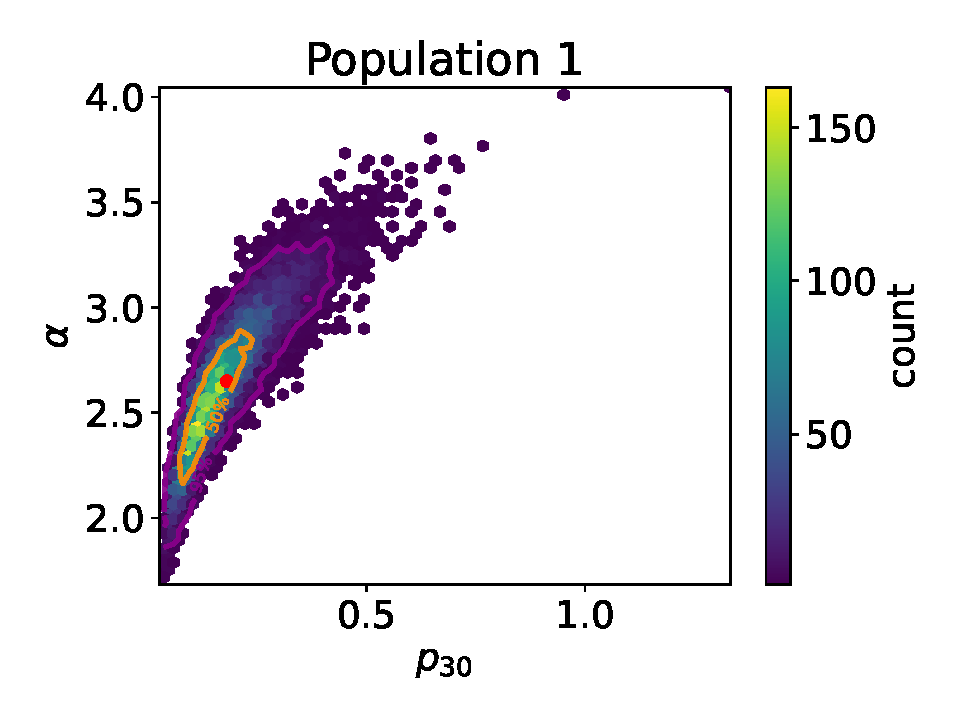
\includegraphics[width=\textwidth]{graphics_tr/fr_pop_1.pdf}
         % \caption{$y=x$}
         % \label{fig:y equals x}
     \end{subfigure}
     \hfill
     \begin{subfigure}[b]{0.325\textwidth}
         \centering
         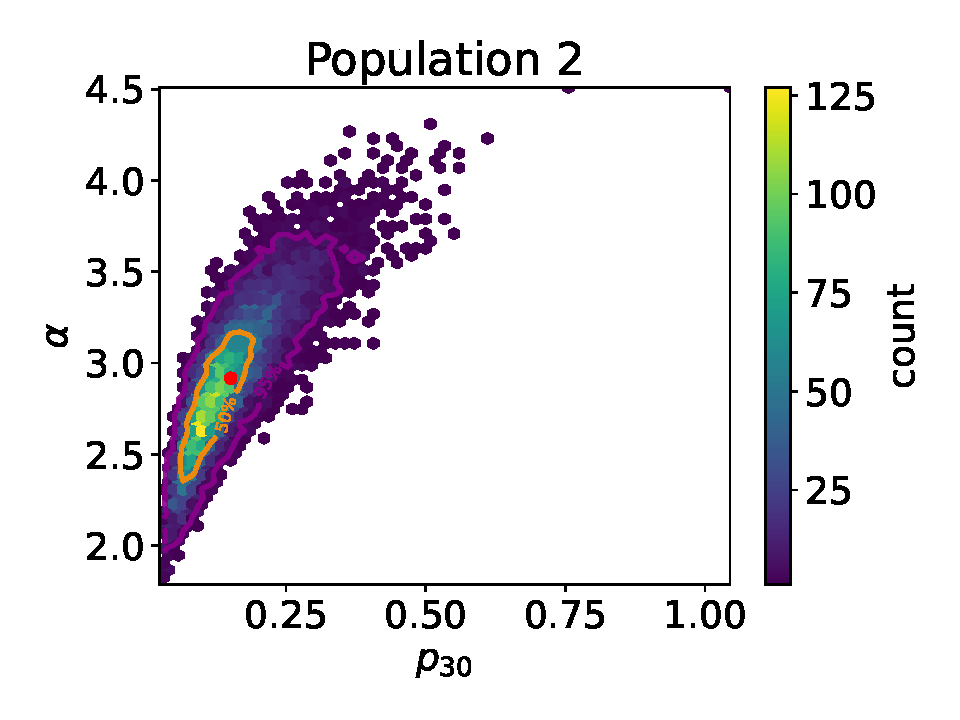
\includegraphics[width=\textwidth]{graphics_tr/fr_pop_2.pdf}
         % \caption{$y=3\sin x$}
         % \label{fig:three sin x}
     \end{subfigure}
     \hfill
     \begin{subfigure}[b]{0.325\textwidth}
         \centering
         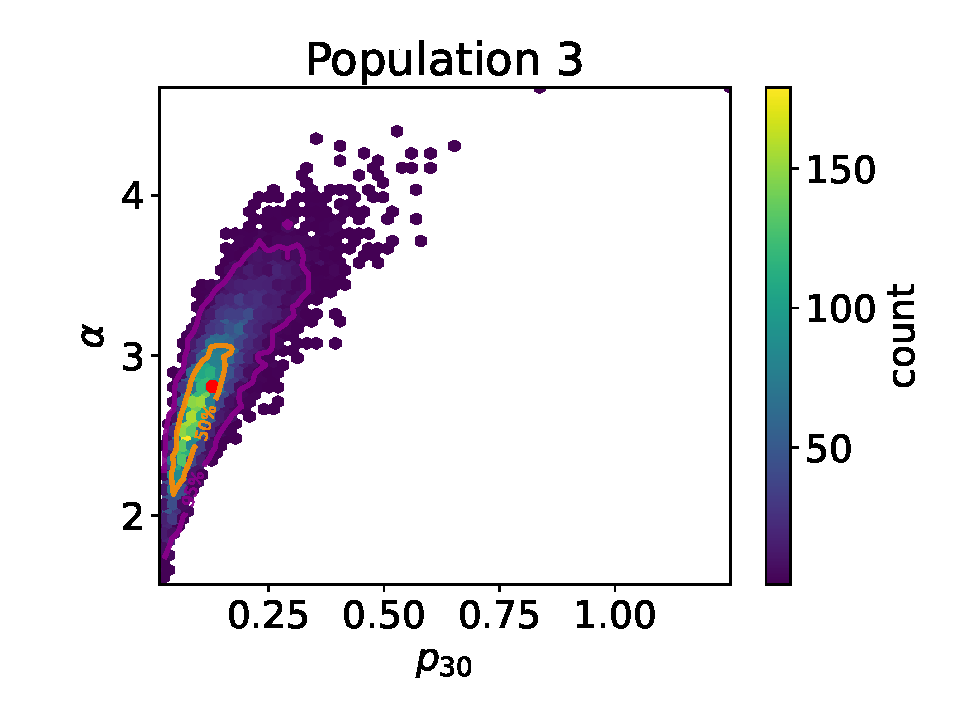
\includegraphics[width=\textwidth]{graphics_tr/fr_pop_3.pdf}
         % \caption{$y=5/x$}
         % \label{fig:five over x}
     \end{subfigure}

     \begin{subfigure}[b]{0.325\textwidth}
         \centering
         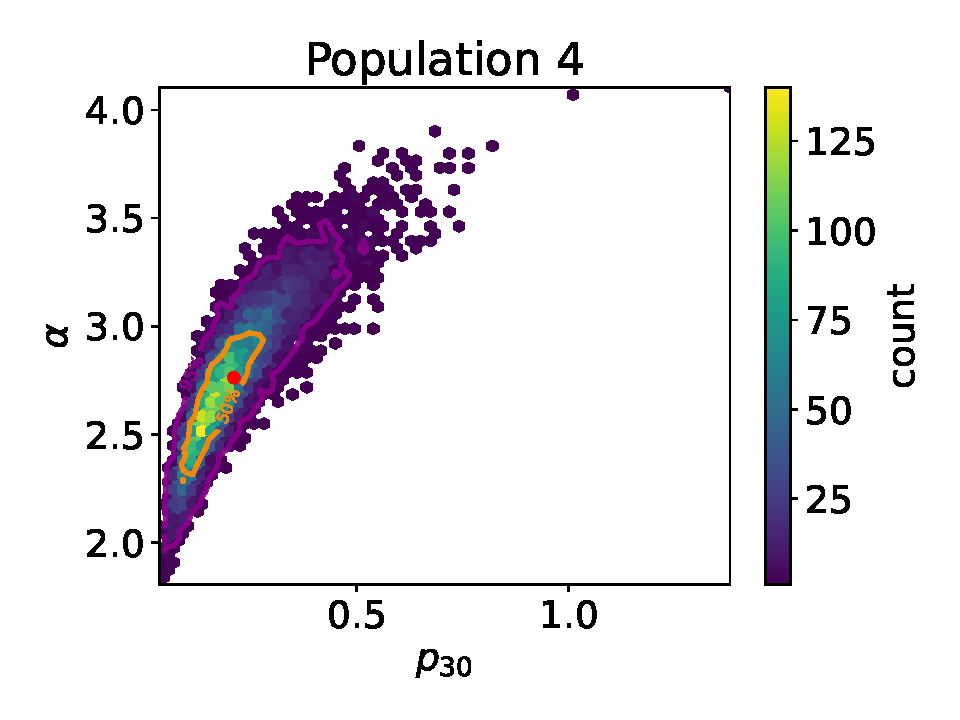
\includegraphics[width=\textwidth]{graphics_tr/fr_pop_4.pdf}
         % \caption{$y=x$}
         % \label{fig:y equals x}
     \end{subfigure}
     \hfil
     \begin{subfigure}[b]{0.325\textwidth}
         \centering
         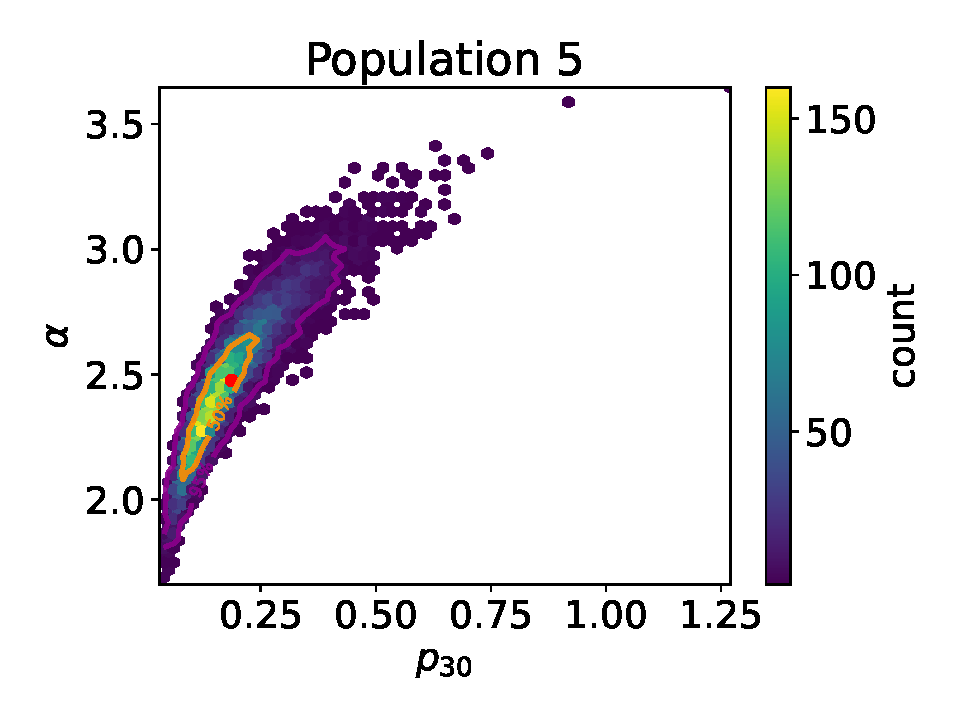
\includegraphics[width=\textwidth]{graphics_tr/fr_pop_5.pdf}
         % \caption{$y=3\sin x$}
         % \label{fig:three sin x}
     \end{subfigure}
        \caption{Posterior distributions of fracture size parameters
        $(p_{30}, \alpha)$ resulting from the Bayesian inversion per fracture
        population.}
        \label{fig:fr_size_distr}
\end{figure}


\begin{figure}[!htb]
     \centering
     \begin{subfigure}[b]{0.325\textwidth}
         \centering
         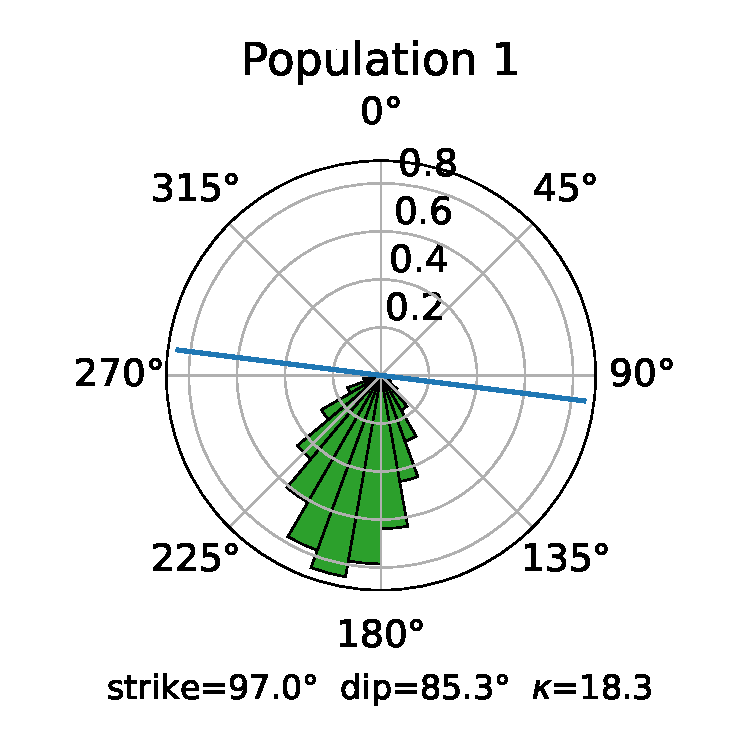
\includegraphics[width=\textwidth]{graphics_tr/fr_rose_1.pdf}
         % \caption{$y=x$}
         % \label{fig:y equals x}
     \end{subfigure}
     \hfill
     \begin{subfigure}[b]{0.325\textwidth}
         \centering
         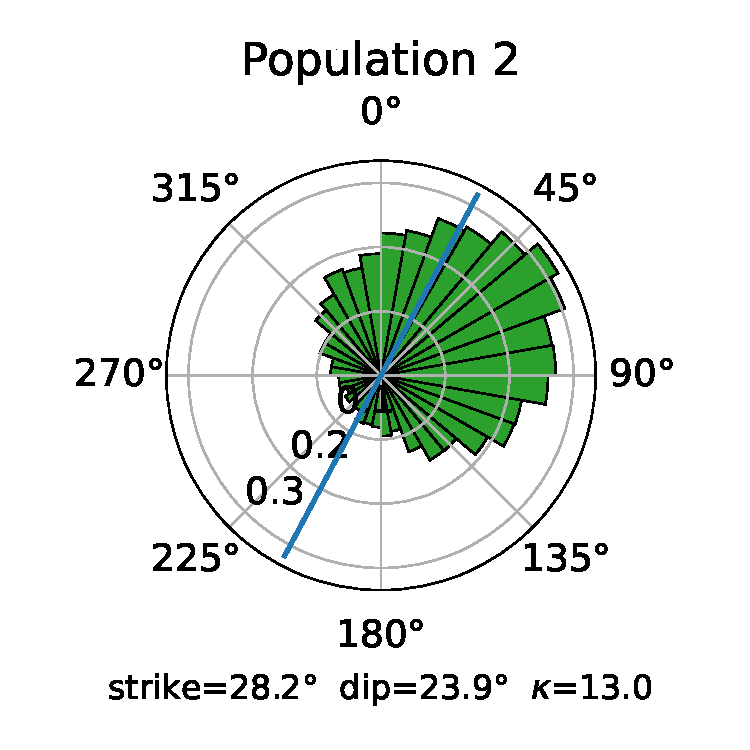
\includegraphics[width=\textwidth]{graphics_tr/fr_rose_2.pdf}
         % \caption{$y=3\sin x$}
         % \label{fig:three sin x}
     \end{subfigure}
     \hfill
     \begin{subfigure}[b]{0.325\textwidth}
         \centering
         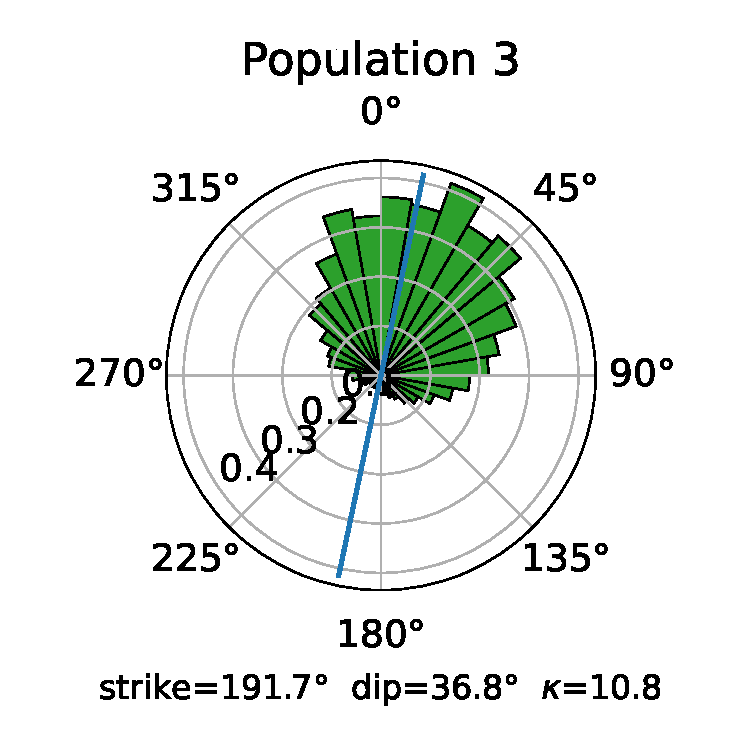
\includegraphics[width=\textwidth]{graphics_tr/fr_rose_3.pdf}
         % \caption{$y=5/x$}
         % \label{fig:five over x}
     \end{subfigure}

     \begin{subfigure}[b]{0.325\textwidth}
         \centering
         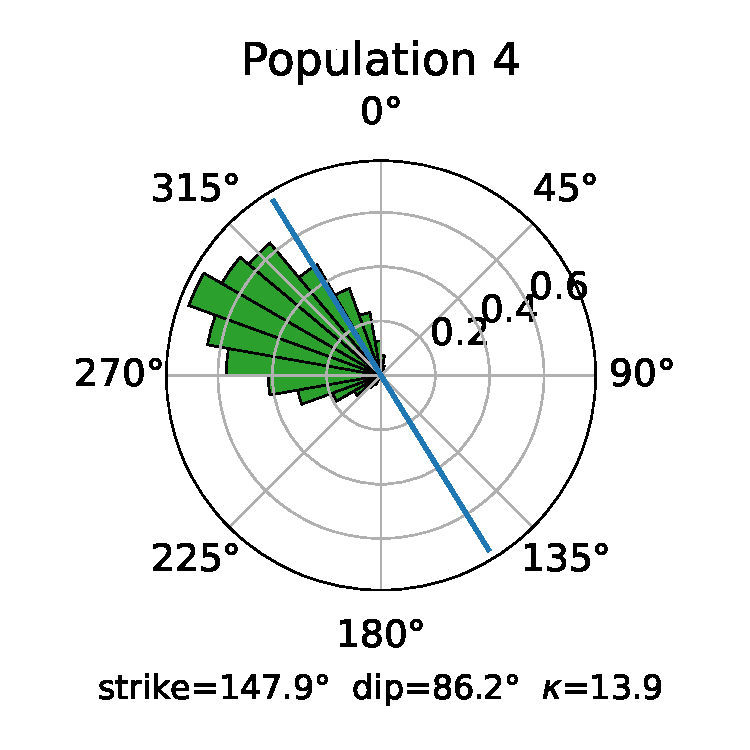
\includegraphics[width=\textwidth]{graphics_tr/fr_rose_4.pdf}
         % \caption{$y=x$}
         % \label{fig:y equals x}
     \end{subfigure}
     \hfil
     \begin{subfigure}[b]{0.325\textwidth}
         \centering
         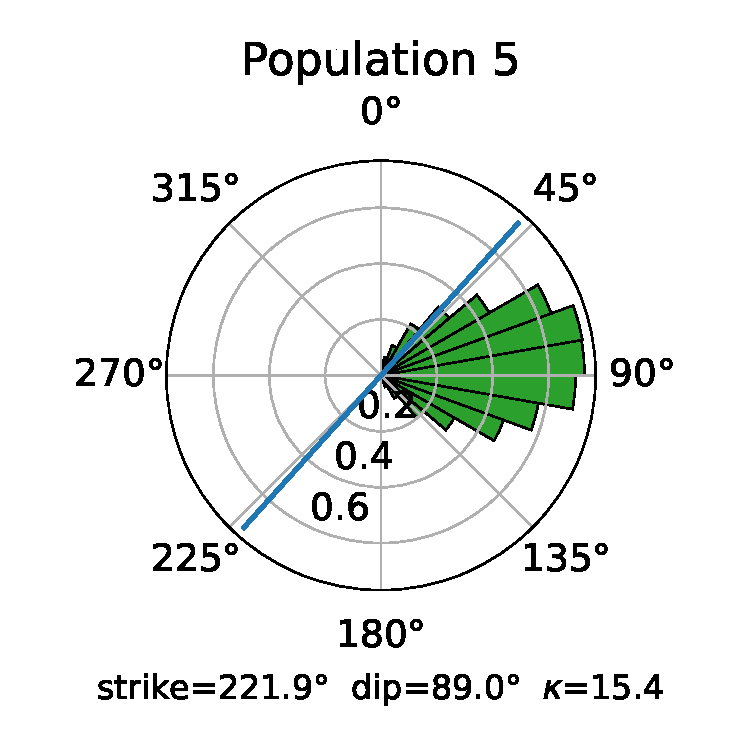
\includegraphics[width=\textwidth]{graphics_tr/fr_rose_5.pdf}
         % \caption{$y=3\sin x$}
         % \label{fig:three sin x}
     \end{subfigure}
        \caption[Strike rose diagrams of fracture orientation by
        von Mises-Fisher distribution per fracture population.]
        {Strike rose diagrams of fracture orientation by von
        Mises-Fisher distribution per fracture population.%
        \protect\footnotemark}
        \label{fig:fr_fisher}
\end{figure}
\footnotetext{\jb{Rose diagrams porvides only information about strike and blue
lines are possibly inconsistent with green histograms. Modify these plots to
use sphere projection of the fracture normals, provides info about both strike
and dip. All populations could possibly be in a single plot distinguished by
color.}}

\paragraph{EDZ parameters}
Based on the analysis in Section~\ref{sec:hm_steady}, we set the outer EDZ
boundary to $\edzRelThick = 1.5$--$2.5$ times the tunnel size. The conductivity
scaling factor is sampled as $\edzPerm \in [0.1,\,100]$
(see \figref{fig:range_conductivity_box}), and the porosity scaling factor as
$\edzPor \in [0.35,\,2.15]$.
A summary of the EDZ parameters is provided in
Table~\ref{tab:param_dfn_edz}.

\paragraph{Matrix properties}
For both the backfill and rock-matrix domains, we prescribe hydraulic
conductivity~$k$, porosity~$\theta$,
effective diffusion coefficient~$d_e$, and longitudinal dispersivity~$\alpha_L$.
For the backfill, mean values and sampling ranges are taken directly from
Section~\ref{sec:transport_pellets}.
For diffusion, we use the mean value representative of neutral species and
cations, while accounting for the larger variability typical of anion-like
tracers.

Rock-matrix properties are based on the review in
Section~\ref{chapter:review}.
The conductivity distribution follows Section~\ref{sec:hydro_cond}, in
particular the analysis of samples from borehole~V--12.
The porosity distribution spans the values reported in
Section~\ref{sec:storativity}, and the effective diffusivity distribution
is based on measurements from borehole~V--12 samples reproduced in
Section~\ref{sec:review_diffusion}.

The dispersivity distribution is derived from the relation
$\alpha_L = I_h\,\Var(\ln K)$, consistent with the macrodispersivity model
introduced in Section~\ref{sec:transport_pellets}, especially
equation~\eqref{eq:dispersivity}.
% var(ln(k))=0.477 for std_log10(k)=0.3
The integral scale $I_h$ is sampled from $0.5$--$5\,\mathrm{m}$, ranging from
the computational element size ($0.5\,\mathrm{m}$)
up to the characteristic size of the smallest discrete fractures
($5\,\mathrm{m}$).

\begin{table}[ht]
    \caption{Summary of DFN and EDZ parameters.}
    \label{tab:param_dfn_edz}
    \hfill
    \begin{minipage}[t]{0.45\textwidth}
        \centering
        \footnotesize
        \renewcommand{\arraystretch}{1.25}
        \begin{tabular}{ccccc}
        \toprule
        \multicolumn{5}{c}{DFN} \\
        \toprule
        $X^*$ & distr. & mean & unit & var \\
        \midrule
        $(p_{30}$, $\alpha)^{(i)}$ & Bayes & -- & -- & -- \\
        % mean_log10: -8.22, std_log10: 0.6
        %$a^{(i)}$ & logN & $0.6$& $\munit{m^2\cdot s^{-1}}$ & $63$ \\
        $a^{(i)}$ & logN & $6\cdot10^{-9}$& $\munit{m^2\cdot s^{-1}}$ & $63$ \\
        % 9.3E-9 geometric mean of repository level values for 6 families in Ohman 2010
        % mean log_10 = -8.03, std log_10 = 0.61 ; there must be some confustion since this
        % match the values reported above.



        % $b^{(i)}$ & logN & $19$& MPa & $2.5$ \\
        $b^{(i)}$ & -- & $3$ & -- & -- \\
        \bottomrule
        \end{tabular}
        $^*$ We denote by $(\cdot)^{(i)}$ the parameters respective to one of
        the fracture population family, $i=0,\ldots,4$.
    \end{minipage}
    \hspace{2em}
    \begin{minipage}[t]{0.45\textwidth}
        \centering
        \footnotesize
        \renewcommand{\arraystretch}{1.25}
        \begin{tabular}{ccccc}
        \toprule
        \multicolumn{5}{c}{EDZ} \\
        \toprule
        $X$ & distr. & mean & unit & var \\
        \midrule
        \(\tilde{w}_e\) & tr. N & $2, [1.5,3]$ & -- & $0.15$ \\
        % mean_log10: 0.5, std_log10: 0.5
        \(\tilde k_e\) & logN & $3.16$ & -- & $31.6$ \\
        % 1.25, 0.3, 0.35, 2.15
        \(\tilde \theta_e\) & tr. N & $1.25, [0.35,2.15]$ & -- & $0.3$ \\
        \bottomrule
        \end{tabular}
    \end{minipage}
    \hfill
\end{table}

\begin{table}[ht]
    \caption{Summary of intact rock and bentonite backfill transport
    parameters.}
    \label{tab:param_matrix_backfill}
    \centering
    \begin{minipage}{0.44\textwidth}
        \centering
        \footnotesize
        \setlength{\tabcolsep}{4pt}
        \renewcommand{\arraystretch}{1.25}
        \begin{tabular}{@{}ccccc@{}}
        \toprule
        \multicolumn{5}{c}{Matrix} \\
        \toprule
        $X$ & dist. & mean & unit & var \\
        \midrule
        % mean_log10: -12.698970004336019, std_log10: 0.1
        $d_r$ & logN & $2 \cdot 10^{-13}$ &
        $\munit{m^2\cdot s^{-1}}$ & $2.00$ \\
        % mean_log10: -12.522878745280337, std_log10: 0.3
        \(k_r\) & logN & $3 \cdot 10^{-13}$ & $\munit{m\cdot s^{-1}}$& $7.94$ \\
        % 0.008, 0.002, 0.001, 0.014
        \(\theta_r\) & tr. N & $0.008,\,[0.001,0.014]$ & -- & $0.002$ \\
        % mean_log10: -0.3010299956639812, std_log10: 0.15
        \(\alpha_{Lr}\) & logN & $0.5$ & $\munit{m}$ & $2.82$ \\
        \bottomrule
        \end{tabular}
    \end{minipage}
    \hfill
    \begin{minipage}{0.44\textwidth}
        \centering
        \footnotesize
        \setlength{\tabcolsep}{4pt}
        \renewcommand{\arraystretch}{1.25}
        \begin{tabular}{@{}ccccc@{}}
        \toprule
        \multicolumn{5}{c}{Backfill} \\
        \toprule
        $X$ & dist. & mean & unit & var \\
        \midrule
        % mean_log10: -11.0, std_log10: 0.3
        $d_b$ & logN & $10^{-11}$ &
        $\munit{m^2\cdot s^{-1}}$ & $7.94$ \\
        % mean_log10: -12.397940008672037, std_log10: 0.26
        \(k_b\) & logN & $3\cdot10^{-13}$ & $\munit{m\cdot s^{-1}}$& $6.03$ \\
        % [0.51, 0.02, 0.45, 0.57]
        \(\theta_b\) & tr. N & $0.51,\,[0.45,0.57]$ & -- & $0.02$ \\
        % mean_log10: -1.08, std_log10: 0.15
        \(\alpha_{Lb}\) & logN & $0.083$ & $\munit{m}$ & $2.82$ \\
        \bottomrule
        \end{tabular}
    \end{minipage}

\end{table}

\FloatBarrier

%%%%%%%%%%%%%%
% TODO:
% - research of similar analysis
% - grafy: menší font popisků, sladit barvy, errorbars v grafech Sobol indexů
